\documentclass{article}
\usepackage{graphicx, soul, amsmath, amssymb, multirow, array, colortbl, float, pgfplots}
\usepackage[dvipsnames]{xcolor}
\usepackage[a4paper, margin=0.8in]{geometry}
\usepackage{fancyhdr} % Paquete para encabezados y pies de página
\usepackage[utf8]{inputenc}
\pgfplotsset{compat=1.18}

% Configuración de soul
\setul{0.5ex}{0.3ex}

% Comandos personalizados
\newcommand{\ulcolor}[2][Red]{\setulcolor{#1}\ul{#2}}
\newcommand*\sepline{%
  \begin{center}
    \rule[1ex]{.5\textwidth}{.5pt}
  \end{center}}

% Configuración de encabezado y pie de página para todas las páginas
\fancypagestyle{main}{
    \fancyhf{} % Limpia encabezados y pies de página
    \fancyhead[C]{Juan Ignacio Elosegui} % Encabezado centrado con tu nombre
    \fancyfoot[R]{\thepage} % Número de página alineado a la derecha en el pie
    \renewcommand{\headrulewidth}{0.4pt} % Línea bajo el encabezado
    \renewcommand{\footrulewidth}{0pt}   % Sin línea en el pie de página
}

% Aplicar el estilo por defecto a todo el documento
\pagestyle{main}

\title{Teoría de las Decisiones $-$ Juegos (Resumen)}
\date{Diciembre 2024}

\begin{document}

    % Primera página con título y encabezado
    \maketitle
    \thispagestyle{main} % Asegura el estilo en la primera página

    \section*{\underline{Módulo 1: Introducción a Juegos y Juegos Simultáneos}}
        \subsection*{Clase I: Introducción y Conceptos Básicos}
            \subsubsection*{Teoría de Juegos}
                La teoría de juegos está dentro de la teoría de las decisiones. Estudia situaciones de interacción estratégica en las cuales los resultados obtenidos no sólo dependen del agente que tomó una decisión, sino también del resto de las decisiones que toman los otros agentes.
                
                La teoría de juegos nos permite analizar situaciones cotidianas o problemas más significativos. \\
                \\
                Hay que entender que en los juegos no juego solo. Mis pagos van a depender de mis decisiones y de las decisiones del resto. Por eso, tengo que tener noción acerca de la interacción que tenemos con los demás y qué quieren ellos también.

                Así como el comportamiento de ellos me afecta a mí, esto también pasa en el sentido contrario. \\
                \\
                En 1971 se hace efectiva la Public Health Cigarette Smoking Act en Estados Unidos, donde se prohíbe la publicidad de cigarrillos en televisión y radio. Se esperaba que las marcas de cigarrillos tengan menos ganancias. \\
                \\
                Antes de la prohibición, las empresas de cigarrillos se encontraban en una situación del Dilema del Prisionero. Las dos empresas (Marlboro y Lucky Strike) invertían en publicidad y obtenían pagos por US\$40 millones. ¿Por qué lo hacían si podían obtener US\$50 millones cuando ninguna de las dos invertía? 
                \begin{table}[h]
                    \centering
                        \begin{tabular}{|c|c|c|c|}
                        \hline
                                                &               & \multicolumn{2}{c|}{\ulcolor[Blue]{Lucky Strike}}                                  \\ \hline
                                                &               & No invertir                           & Invertir                              \\ \hline
                        \multirow{2}{*}{\ulcolor[Red]{Marlboro}} 
                                                & No invertir   & \ulcolor[Red]{50}, \ulcolor[Blue]{50} & \ulcolor[Red]{50}, \ulcolor[Blue]{50} \\ \cline{2-4} 
                                                & Invertir      & \ulcolor[Red]{50}, \ulcolor[Blue]{50} & \ulcolor[Red]{50}, \ulcolor[Blue]{50} \\\hline
                        \end{tabular}
                    \caption{Juego representado de forma normal}
                \end{table} \\
                Cuando se prohibió que estas marcas publicitaran sus cigarrillos, las ganancias de estas subieron a 50 millones.
            \subsubsection*{Deciciones Individuales, Azar y Juegos}
                Una \textbf{decisión individual} es cuando realizo una acción pero no necesito tener en cuenta las respuestas de los demás. \\
                \\
                En ciertos casos, los resultados de mis decisiones pueden estar mediadas por el \emph{azar} (o la incertidumbre) relacionado al contexto pero no las convierte en decisiones de orden estratégico. \\
                \\
                Una \textbf{estrategia} es cuando tengo en cuenta la respuesta de los otros jugadores y también considero la reacción de los otros sobre mis acciones.
            \subsubsection*{Elementos de un Juego}
                \begin{itemize}
                    \item Jugadores
                        \subitem Los que intervienen en el juego.
                    \item Estrategias
                        \subitem Las opciones disponibles para los jugadores.
                    \item Pagos/preferencias
                        \subitem Mayores pagos numéricos estarán asociados a resultados que son mejores en el sistema de ordenamiento del jugador (preferencias).
                    \item Racionalidad
                        \subitem El jugador calcula la estrategia que mejor le sirve para sus intereses.
                    \item Información común sobre las reglas
                        \subitem Los jugadores saben quiénes juegan, qué estrategias tienen disponibles y los pagos de cada combinación posible. Si alguno no se cumple aparece la asimetría de la información.
                    \item Equilibrio
                        \subitem Cada jugador está usando la estrategia que es la mejor respuesta a las estrategias de los otros jugadores.
                \end{itemize}
        \subsection*{Clase II: Juegos Simultáneos y Dominancia}
            \subsubsection*{Juegos Simultáneos/Estáticos}
                \begin{itemize}
                    \item Estos juegos son simultáneos porque los jugadores juegan al mismo tiempo ó juegan en diferentes momentos del tiempo, pero sin saber lo que otros jugaron.
                    \item Son one-shot porque se juegan de a una sola vez, no se repiten.
                    \item En estos juegos, tomar una estrategia es lo mismo que tomar una acción.
                    \item Son juegos de información completa.
                \end{itemize}
            \subsubsection*{Dominancia}
                \begin{table}[h]
                    \centering
                        \begin{tabular}{|c|c|c|c|}
                        \hline
                                                &               & \multicolumn{2}{c|}{\ulcolor[Blue]{Jugador B}} \\ \hline
                                                &               & Arriba & Abajo \\ \hline
                        \multirow{3}{*}{\ulcolor[Red]{Jugador A}} 
                                                & Rojo & \ulcolor[Red]{1}, \ulcolor[Blue]{3} & \ulcolor[Red]{8}, \ulcolor[Blue]{2} \\ \cline{2-4} 
                                                & Verde & \ulcolor[Red]{6}, \ulcolor[Blue]{2} & \ulcolor[Red]{10}, \ulcolor[Blue]{1}\\\cline{2-4}
                                                & Azul & \ulcolor[Red]{5}, \ulcolor[Blue]{4} & \ulcolor[Red]{9}, \ulcolor[Blue]{3}\\\hline
                        \end{tabular}
                    \caption{Juego representado de forma normal}
                \end{table}
                Si yo fuera el \ulcolor[Red]{Jugador A}, jugaría verde siempre. Porque los pagos que me da esta opción son mayores sin importar qué elija el \ulcolor[Blue]{Jugador B}. \\
                Si yo fuera el \ulcolor[Blue]{Jugador B}, jugaría arriba, porque los pagos en esta opción, en general, son mayores o iguales que jugar abajo. \\
                Para el \ulcolor[Red]{Jugador A}, si juega verde, sabe que los pagos con esa estrategia son todos mayores que los pagos de rojo y azul \(\{(6 > 5 > 1), (10, 9, 8)\}\). Lo mismo pasa para el \ulcolor[Blue]{Jugador B}, todos los pagos con la estrategia de jugar arriba son mayores que los pagos de jugar abajo: \(\{(3 > 2), (2 > 1), (4 > 3)\}\). \\
                \\
                Una estrategia es \textbf{estrictamente dominante} si siempre proporciona un mayor pago (estrictamente) que cualquier otra estrategia alternativa, \emph{independientemente de lo que haga el otro jugador/jugadores}. Una estrategia es estrictamente dominante para un jugador si todas las otras estrategias están dominadas por esa estrategia dominante. \\
                \\
                Si todos los jugadores tienen una estrategia estrictamente dominante, entonces si cada jugador juega su estrategia estrictamente dominante se llegará a un equilibrio en estrategias estrictamente dominantes (EEED).
            \subsubsection*{El Dilema del Prisionero}
                \begin{table}[h]
                    \centering
                        \begin{tabular}{|c|c|c|c|}
                        \hline
                                                & & \multicolumn{2}{c|}{\ulcolor[Blue]{Jugador B}}  \\ \hline
                                                & & Confesar & Negar  \\ \hline
                        \multirow{2}{*}{\ulcolor[Red]{Jugador A}} 
                                                & Confesar & \ulcolor[Red]{-10}, \ulcolor[Blue]{-10} & \ulcolor[Red]{-1}, \ulcolor[Blue]{-25} \\ \cline{2-4} 
                                                & Negar & \ulcolor[Red]{-25}, \ulcolor[Blue]{-1} & \ulcolor[Red]{-3}, \ulcolor[Blue]{-3} \\\hline
                        \end{tabular}
                    \caption{Juego de El Dilema del Prisionero}
                \end{table}
                En este juego:
                \begin{itemize}
                    \item Los jugadores pueden Confesar o Negar.
                    \item Cada jugador tiene una estrategia estrictamente dominante.
                    \item La solución de equilibrio bajo dominancia no es un Óptimo de Pareto porque existe un resultado alternativo del juego en el que los dos estarían mejor, (\ulcolor[Red]{-3}, \ulcolor[Blue]{-3}), pero la falta de cooperación hace que no se pueda alcanzar porque están en dos habitaciones distintas.
                \end{itemize}
                Un Óptimo de Pareto es un resultado eficiente porque no existe otro resultado posible que mejore la posición de uno sin empeorar la posición del otro.
                \begin{table}[h]
                    \centering
                    \begin{tabular}{|c|c|c|c|}
                        \hline
                            & Left  & Center    & Right \\ \hline
                        Up  & 1,0   & 1,2       & 0,1   \\ \hline
                        Down& 0,3   & 0,1       & 2,0   \\ \hline
                    \end{tabular}
                    \caption{Estrategias para J1 y J2}
                \end{table}
                \\
                En este caso, podemos ver que el Jugador 1 (el que tiene las opciones Up y Down), no tiene una estrategia estrictamente dominante. Esto es porque, si bien le conviene jugar Up cuando el Jugador 2 juega Left y Center, no le convendrá jugar Up cuando el Jugador 2 juega Right. Por lo que el Jugador 1 no tiene una estrategia dominante, dado que no existe una estrategia que ofrezca mejores pagos que cualquier otra estrategia alternativa, sin importar lo que jugó el Jugador 2. \\
                El Jugador 2 jugará Center si el Jugador 1 juega Up, pero tendrá que jugar Left si el Jugador 1 juega Down. Habiendo dicho esto, no tiene una estrategia estrictamente dominante. \\
                \\
                Informalmente, una estrategia de un jugador está \textbf{estrictamente dominada} si existe otra estrategia posible que proporciona al jugador un pago mayor independientemente de lo que hagan los demás jugadores.
            \subsubsection*{Eliminación Sucesiva de Estrategias}
                Si una estrategia (ej: A) es estrictamente dominada por otra (ej: B), no necesariamente implica que B sea estrictamente dominante. ¿Por qué? En el juego podría haber otras estrategias que no estén dominadas por B. \\
                \\
                Las estrategias que están estrictamente dominadas pueden ser eliminadas de juego, reduciendo el tamaño del tablero, porque un jugador racional no va a jugar una estrategias estrictamente dominadas. Podemos predecir el resultado final del juego siguiendo el proceso de \emph{Eliminación Sucesiva de Estrategias Estrictamente Dominadas (ESEED)}.

                El orden de la eliminación no importa cuando eliminamos estrategias estrictamente dominadas de manera iterativa o sucesiva. \emph{No funciona cuando eliminamos estrategias débilmente dominadas}. \\
                \\
                Si queremos eliminar estrategias \emph{débilmente dominadas} es distinto el proceso. Estas no se pueden eliminar, y, si lo hacemos, el orden de eliminación puede afectar el resultado final del juego. Este procedimiento nos puede llevar a descartar un equilibrio de Nash válido. 
            \subsubsection*{Eliminación Sucesiva de Estrategias}
                Las \textbf{estrategias racionalizables} son \emph{aquellas que quedan} luego de hacer la eliminación sucesiva de estrategias estrictamente dominadas. Se les dice "racionalizables" porque cualquier jugador racional querría jugar esas estrategias que quedan.
        \subsection*{Clase III: Juegos Simultáneos y Equilibrio de Nash (Parte 1)}
            \subsubsection*{Equilibrio de Nash}
                \begin{table}[H]
                    \centering
                    \begin{tabular}{|c|c|c|c|c|}
                        \hline
                        & \textbf{W} & \textbf{X} & \textbf{Y} & \textbf{Z} \\ \hline
                        \textbf{A} & \textcolor{red}{0}, \textcolor{blue}{1} & \textcolor{red}{0}, \textcolor{blue}{1} & \textcolor{red}{1}, \textcolor{blue}{0} & \textcolor{red}{3}, \textcolor{blue}{2} \\ \hline
                        \textbf{B} & \textcolor{red}{1}, \textcolor{blue}{2} & \textcolor{red}{2}, \textcolor{blue}{2} & \textcolor{red}{4}, \textcolor{blue}{0} & \textcolor{red}{0}, \textcolor{blue}{2} \\ \hline
                        \textbf{C} & \textcolor{red}{2}, \textcolor{blue}{1} & \textcolor{red}{0}, \textcolor{blue}{1} & \textcolor{red}{1}, \textcolor{blue}{2} & \textcolor{red}{1}, \textcolor{blue}{0} \\ \hline
                        \textbf{D} & \textcolor{red}{3}, \textcolor{blue}{0} & \textcolor{red}{1}, \textcolor{blue}{0} & \textcolor{red}{1}, \textcolor{blue}{1} & \textcolor{red}{3}, \textcolor{blue}{1} \\ \hline
                    \end{tabular}
                    \caption{Matriz de estrategias de Jugador A y Jugador B. El \textcolor{Red}{Jugador A} representa las filas, y el \textcolor{Blue}{Jugador B} representa las columnas.}
                \end{table}
                Hay veces en los que la dominancia no me va a ayudar a resolver un juego (por ejemplo, si tengo muchas estrategias racionalizables). Para eso quiero encontrar el \textbf{equilibrio de Nash}. \\
                \\
                Si queremos encontrar este equilibrio especial, primero tenemos que saber lo que es la \textbf{mejor respuesta}. La mejor respuesta de un jugador es una estrategia que maximiza sus pagos, \emph{dado lo que hace el resto de los jugadores}. La mejor respuesta a la estrategia de un rival puede no ser única. \\
                \\
                Un equilibrio de Nash (EN) es una combinación de estrategias (una estrategia para cada jugador) tal que, si sus oponentes eligen la estrategia correspondiente a ese equilibrio, ningún jugador podría recibir un pago mayor si eligiese moverse hacia otra estrategia.

                En un EN, \emph{cada jugador está jugando su mejor respuesta dado lo que juegan los otros}, por lo que no existen incentivos a desviarse. \\
                \\
                Para encontrar el equilibrio de Nash debo hacer lo siguiente:
                \begin{enumerate}
                    \item ¿Cuál es mi mejor respuesta para cada estrategia que juegue mi adversario? Hacer esto para todos los jugadores y para todas las estrategias.
                    \item Analizando las mejores respuestas de todos, queremos buscar las intersecciones.
                    \item Si no hay intersecciones, el juego no tiene un EN en estrategias puras.
                \end{enumerate}
                Volviendo al cuadro, busco los EN:
                \begin{table}[H]
                    \centering
                    \begin{tabular}{|c|c|c|c|c|}
                        \hline
                                    & \textbf{W} & \textbf{X} & \textbf{Y} & \textbf{Z} \\ \hline
                        \textbf{A}  & 0, 1 & 0, 1 & 1, 0 & \ulcolor[Red]{3}, \ulcolor[Blue]{2} \\ \hline
                        \textbf{B}  & 1, \ulcolor[Blue]{2} & \ulcolor[Red]{2}, \ulcolor[Blue]{2} & \ulcolor[Red]{4}, 0 & 0, \ulcolor[Blue]{2} \\ \hline
                        \textbf{C}  & 2, 1 & 0, 1 & 1, \ulcolor[Blue]{2} & 1, 0 \\ \hline
                        \textbf{D}  & \ulcolor[Red]{3}, 0 & 1, 0 & 1, \ulcolor[Blue]{1} & \ulcolor[Red]{3}, \ulcolor[Blue]{1} \\ \hline
                    \end{tabular}
                    \caption{Matriz de estrategias de Jugador A y Jugador B. El Jugador A representa las filas, y el Jugador B representa las columnas.}
                \end{table}
                Concluyo que los EN \(= \{(B,X);(D,Z)\}\). Notar que son las combinaciones de columnas y filas que tienen los dos las mejores respuestas. \\
                \begin{itemize}
                    \item En un EN no existen incentivos al desvío. En ese punto, los jugadores están satisfechos con sus decisiones.
                    \item No está asegurado que sea un Pareto eficiente.
                    \item Una estrategia estrictamente dominada NO puede formar parte de un EN.
                    \item Una estrategia débilmente dominada sí puede estar.
                \end{itemize}
            \subsubsection*{Equilibrios Múltiples}
                En un juego puede haber un único EN (como en el dilema del prisionero) o múltiples EN. Esto puede verse en los juegos llamados \textbf{juegos de coordinación}. \\
                \\
                En el juego de \textbf{la caza del ciervo}, se presenta el siguiente contexto:
                \begin{itemize}
                    \item Si un jugador decide cazar una liebre consigue hacerlo con certeza, mientras que para cazar el ciervo se necesita del esfuerzo de ambos (todos) los jugadores.
                    \item Cada jugador prefiere obtener una porción del ciervo antes que la liebre.
                    \item Intentar cazar el ciervo en soledad es el peor escenario.
                \end{itemize}
                \begin{table}[H]
                    \centering
                        \begin{tabular}{|c|c|c|c|}
                        \hline
                        & & \multicolumn{2}{c|}{Jugador 2} \\ \hline
                                                & & Ciervo & Conejo \\ \hline
                        \multirow{2}{*}{\ulcolor[Red]{Jugador 1}} 
                                                & Ciervo & 2, 2 & 0, 1 \\ \cline{2-4} 
                                                & Conejo & 1, 0 & 1,1 \\ \hline
                        \end{tabular}
                    \caption{Juego de la caza del ciervo}
                \end{table}
                Si resuelvo el juego:
                \begin{table}[H]
                    \centering
                        \begin{tabular}{|c|c|c|c|}
                        \hline
                        & & \multicolumn{2}{c|}{Jugador 2} \\ \hline
                                                & & Ciervo & Conejo \\ \hline
                        \multirow{2}{*}{Jugador 1} 
                                                & Ciervo & \ulcolor[Red]{2}, \ulcolor[Blue]{2} & 0, 1 \\ \cline{2-4} 
                                                & Conejo & 1, 0 & \ulcolor[Red]{1}, \ulcolor[Blue]{1} \\ \hline
                        \end{tabular}
                    \caption{Juego de la caza del ciervo resuelto}
                \end{table}
                Hay dos EN, pero solo uno de ellos es eficiente (que sería (2,2) porque es lo mejor que pueden conseguir). Además, esperarías que los dos jugadores colaboren para cazar el ciervo y se lleven una porción grande los dos. Si los jugadores fueran individualistas, les aseguraría ir por el conejo cada uno por su lado, dándoles un nivel mínimo de bienestar.
            \subsubsection*{Juegos de Suma Cero}
                Presento el juego de \textbf{Matching Pennies}. \\
                Si ambos coinciden, A gana (+1) y B pierde (-1). Si eligieron distinto, A pierde (-1) y B gana (+1)
                \begin{table}[H]
                    \centering
                        \begin{tabular}{|c|c|c|c|}
                        \hline
                        & & \multicolumn{2}{c|}{\textcolor{Blue}{Jugador 2}} \\ \hline
                                                & & Cara & Cruz \\ \hline
                        \multirow{2}{*}{\textcolor{Red}{Jugador 1}} 
                                                & Cara & \ulcolor[Red]{1}, -1 & -1, \ulcolor[Blue]{1} \\ \cline{2-4} 
                                                & Cruz & -1, \ulcolor[Blue]{1} & \ulcolor[Red]{1}, -1 \\ \hline
                        \end{tabular}
                    \caption{Juego de la caza del ciervo resuelto}
                \end{table}
                Frente a cualquier combinación de estrategias puras, siempre hay uno de los dos jugadores que tiene incentivos a cambiar su elección. No hay EN en estrategias puras. \\
                \\
                Cada estrategia que es parte de un EN es una estrategia racionalizable. Entonces, podemos restringir la búsqueda del EN a estrategias racionalizables.
        \subsection*{Clase IV: Juegos Simultáneos y Equilibrio de Nash (Parte 2)}
            \subsubsection*{Estrategias Continuas}
                En las \textbf{estrategias continuas}, los jugadores eligen el nivel del una variable continua, por lo que no se puede representar el juego de una forma normal. 
            \subsubsection*{Duopolio de Bertrand}
                En esta competencia entre dos firmas, las decisiones estratégicas se basan en elegir el precio único del menú de forma simultánea: \\
                \\
                ``La Pastelería de Maru'': \(p_{1}\) \\
                ``La Pastelería de Pani'': \(p_{2}\) \\
                \\
                La demanda del bien está dada por \(Q = 1000-p\), donde \(Q = q_{1}+q_{2}\). Dado un cierto precio \(p\), los consumidores demandan \(1000-p\) menúes. \\
                \\
                El costo marginal es constante e igual a \(\mathdollar 100\) por unidad. \\
                \\
                Esto determina que:
                \begin{itemize}
                    \item Si \(p_{1} = p_{2}\), se dividen el mercado de clientes a la mitad, porque cada pastelería vende una cantidad de \(\frac{1000-p}{2}\).
                    \item Si las pastelerías eligen precios distintos, los consumidores le compran sólo a la que tiene el precio más bajo, y su demanda pasaría a ser \(1000-p\) y la demanda de la otra pastelería sería 0.
                \end{itemize}
                Si buscamos los pagos de cada pastelería nos quedaría así:
                \[
                    Beneficios_{i} =
                    \begin{cases} 
                    0 & \text{si } p_{i} > p_{j} \\ 
                    \frac{(1000p_{i})(p_{i}-100)}{2} & \text{si } p_{i} = p_{j} \\
                    (1000-p_{i})(p_{i}-100) & \text{si } p_{i} < p_{j}
                    \end{cases}
                \]
                Hay que encontrar la intersección de las mejores respuestas para que no haya incentivos al desvío. Las estrategias de las pastelerías son \(E_{i} = [0, \infty)\).
                \begin{itemize}
                    \item Si \(p_{i} \vee p_{j} < 100\) se va a dar un desvío, porque la firma que vende a ese precio está obteniendo pérdidas y podría estar mejor sin producir. Por lo tanto, cierra.
                    \item Si \(p_{j} > p_{i} \geq 100\) se va a dar un desvío, porque la firma \(j\) puede aumentar sus ganancias (que antes eran 0) al elegir un precio entre 100 y \(p_{i}\).
                    \item Si \(p_{j} = p_{i} > 100\) se va a dar un desvío, porque cada firma obtiene la mitad de la demanda del mercado, pero podría obtener toda la demanda si baja su precio un poco.
                    \item Si \(p_{j} = p_{i} = 100\) las firmas no pueden aumentar sus ganancias al bajar los precios. Entonces, no hay incentivos al desvío y es un EN.
                \end{itemize}
                Este resultado se conoce como la paradoja de Bertrand: ¿cómo es que se alcanza el resultado de un mercado de competencia perfecta en un mercado donde hay nada más que dos oferentes?. La paradoja se puede resolver si decimos como supuestos que cada empresa vende un producto homogéneo idéntico y que cada empresa puede cubrir toda la demanda si elimina a su competidor.
    \section*{\underline{Módulo 2: Estrategias Mixtas}}
        \subsection*{Clase V: Estrategias Mixtas y Equilibrio de Nash (Parte 1)}
            \subsubsection*{Estrategias Mixtas}
                El siguiente cuadro es un análisis que se hizo en 1417 penales de la FIFA y muestra los porcentajes en los que se terminaba en gol.
                \begin{table}[H]
                    \centering
                        \begin{tabular}{|c|c|c|c|}
                        \hline
                        & & \multicolumn{2}{c|}{\textcolor{Blue}{Arquero}} \\ \hline
                                                & & Izquierda & Derecha \\ \hline
                        \multirow{2}{*}{\textcolor{Red}{Jugador}} 
                                                & Izquierda & 58, 42 & 95, 5 \\ \cline{2-4} 
                                                & Derecha & 93, 7 & 70, 30 \\ \hline
                        \end{tabular}
                    \caption{Juego de los penales (con estrategias puras)}
                \end{table}
                Si fuera el jugador, patearía a la izquierda si el arquero se tira a la derecha. Si se tira a la izquierda, entonces pateo a la derecha. \\
                \\
                Si sé que el arquero se va a tirar siempre a la derecha, ni en pedo pateo a la derecha también. Si el arquero sabe que voy a patear siempre a la derecha, entonces sí se tirará a la derecha. Estas son \emph{elecciones sistemáticas}, y, si decido en base a esto, el otro jugador puede aprovecharse y perjudicarme. \\
                \\
                Si quiero evitar que mis decisiones sean aprovechadas por el otro rival, debo jugar una \textbf{estrategia mixta}, que es randomizar la elección entre estrategias puras para que no sea sistemática.

                Tengo que encontrar la mejor combinación de estrategias puras. La mejor combinación será \emph{la que brinde el mayor pago}. \\
                \\
                A diferencia de las estrategias mixtas, las \textbf{estrategias puras} son estrategias a las cuales un jugador elige con una probabilidad de 1 y se les asigna una probabilidad 0 al resto de las estrategias. \\
                En estrategias mixtas, un jugador le asigna una probabilidad \(p\) a la estrategia ``izquierda'' y una probabilidad de \(1-p\) a la estrategia ``derecha''. Claramente, \(0 \leq p \leq 1\). La decisión de \(p\) y \(1-p\) se llama \(p_{mix}\) del jugador. \\
                \\
                El juego entonces pasaría a estar así:
                \begin{table}[H]
                    \centering
                        \begin{tabular}{|c|c|c|c|}
                        \hline
                        & & \multicolumn{2}{c|}{\textcolor{Blue}{Arquero}} \\ \hline
                                                & & Izquierda ($q$) & Derecha ($1-q$) \\ \hline
                        \multirow{2}{*}{\textcolor{Red}{Jugador}} 
                                                & Izquierda ($p$) & 58, 42 & 95, 5 \\ \cline{2-4} 
                                                & Derecha ($1-p$) & 93, 7 & 70, 30 \\ \hline
                        \end{tabular}
                    \caption{Juego de los penales (con estrategias mixtas)}
                \end{table}
                Si quisiera resolver esto, quiero encontrar los puntos de equilibrio tanto del jugador como del arquero. \\
                \(PE_{Izquierda} = 58q + 95(1-q)\) \\
                \(PE_{Derecha} = 93q + 70(1-q)\) \\
                Notar que los pagos esperados del jugador dependen de $q$ porque el arquero decide a dónde tirarse. \\
                En una situación de equilibrio, \(PE_{Izquierda} = PE_{Derecha}\) \\
                \(\implies 58q + 95(1-q) = 93q + 70(1-q)\) \\
                \(\implies 58q + 95-95q = 93q + 70-70q\) \\
                \(\implies 58q - 95q + 70q - 93q = -95 + 70\) \\
                \(\implies -60q= -25\) \\
                \(\implies 60q= 25\) \\
                \(\implies q = \frac{25}{60}\) \\
                \(\implies q = \frac{5}{12}\) \\
                \(\therefore q = \frac{5}{12} \wedge 1-q = \frac{7}{12}\) \\
                \(\therefore q \approx 0,417 \wedge 1-q \approx 0,583 \) Son los puntos de equilibrio del jugador. \\
                \\
                \(PE_{Izquierda} = 42p + 7(1-p)\) \\
                \(PE_{Derecha} = 5p + 30(1-p)\) \\
                En una situación de equilibrio, \(PE_{Izquierda} = PE_{Derecha}\) \\
                \(\implies 42p + 7(1-p) = 5p + 30(1-p)\) \\
                \(\implies 42p + 7-7p = 5p + 30-30p\) \\
                \(\implies 42p-7p+30p-5p = 30-7\) \\
                \(\implies 72p-12p = 23\) \\
                \(\implies 60p = 23\) \\
                \(\implies p = \frac{23}{60}\) \\
                \(\implies p = \frac{23}{60} \wedge 1-p = \frac{37}{60}\) \\
                \(\therefore p \approx 0,383 \wedge 1-p \approx 0,617\) \\
                \\
                Si graficamos las mejores respuestas de los jugadores:
                \[
                    MR_{Arquero}(p_{mix}Jugador) =
                    \begin{cases} 
                    q = 0 & \text{si } p < 0,383 \\ 
                    \text{cualquier $q_{mix}$ es indiferente} & \text{si } p = 0,383 \\
                    q = 1 & \text{si } p > 0,383
                    \end{cases}
                \]
                \[
                    MR_{Jugador}(q_{mix}Arquero) =
                    \begin{cases} 
                    p = 0 & \text{si } q < 0,417 \\ 
                    \text{cualquier $p_{mix}$ es indiferente} & \text{si } q = 0,417 \\
                    p = 1 & \text{si } q > 0,417
                    \end{cases}
                \]
            \subsubsection*{Equilibrio de Nash}
                \begin{center}
                    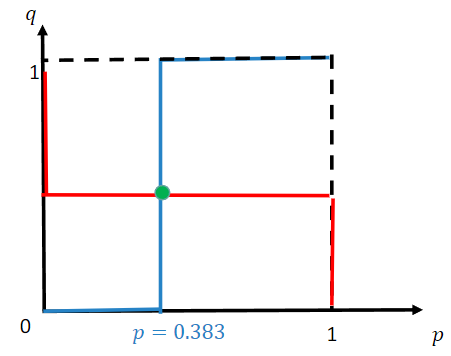
\includegraphics[width=0.8 \linewidth]{figs/mixtas.png}
                \end{center}
                La intersección de los puntos de indiferencia de los jugadores será el EN en estrategias mixtas. Con sólo calcular los puntos de indiferencia, como fue \(PE_{Izquierda} = PE_{Derecha}\), se encuentra el EN. \\
                EN = \(\{(p = 0,383;1-p = 0.617), (q = 0,417; 1-q = 0,583)\}\) \\
                \\
                Todo juego finito tiene -al menos- un equilibrio de Nash en estrategias puras o mixtas.
        \subsection*{Clase VI: Estrategias Mixtas (Parte 2)}
            \subsubsection*{Estrategias Mixtas y Dominancia Estricta}
                \begin{table}[H]
                    \centering
                        \begin{tabular}{|c|c|c|c|}
                        \hline
                        & & \multicolumn{2}{|c|}{\textcolor{Blue}{Columna}} \\ \hline
                                                & & L & R \\ \hline
                        \multirow{2}{*}{\textcolor{Red}{Fila}} 
                                                & U & 3, 0 & 0, 1 \\ \cline{2-4} 
                                                & M & 0, 0 & 3, 1 \\ \cline{2-4}
                                                & D & 1, 1 & 1, 0 \\ \hline
                        \end{tabular}
                \end{table}
                \begin{itemize}
                    \item No hay estrategias puras estrictamente dominadas.
                    \item D no está estrictamente dominada por las otras estrategias puras para el jugador Fila. Ni siquiera D es mejor respuesta para alguna jugada del jugador Columna.
                \end{itemize}
                Supongamos que las creencias del jugador 1 son tales que su \(p_{mix} = (0,5;0,5;0)\). ¿Cuál es el pago esperado de esta estrategia?
                \begin{table}[H]
                    \centering
                        \begin{tabular}{|c|c|c|c|}
                        \hline
                        & & \multicolumn{2}{|c|}{\textcolor{Blue}{Columna}} \\ \hline
                                                & & L & R \\ \hline
                        \multirow{2}{*}{\textcolor{Red}{Fila}} 
                                                & U \textcolor{red}{(0,5)}& 3, 0 & 0, 1 \\ \cline{2-4} 
                                                & M \textcolor{red}{(0,5)}& 0, 0 & 3, 1 \\ \cline{2-4}
                                                & D \textcolor{red}{(0)}& 1, 1 & 1, 0 \\ \cline{2-4}
                                                & Mixta & 1.5, - & 1.5, - \\ \hline
                        \end{tabular}
                \end{table}
                D es estrictmente dominada por la estrategia mixta. De acá en más, puedo descartar esta estrategia (porque no la voy a tener en consideración). Concluimos que (M, R) es el único resultado que sobrevive a la eliminación sucesiva de estrategias estrictamente dominadas. \\
                \\
                ¿Cómo generalizamos la búsqueda de estrategias mixtas que dominen estrictamente a una pura? \\
                \begin{enumerate}
                    \item Consideramos el caso general \(p_{mix} = (p;1-p;0)\).
                    \item Necesitamos que los pagos esperados del $p_{mix}$ sean mayores que los pagos de D frente a todas las estrategias puras del jugador Columna.
                \end{enumerate}
                \begin{table}[H]
                    \centering
                        \begin{tabular}{|c|c|c|c|}
                        \hline
                        & & \multicolumn{2}{|c|}{\textcolor{Blue}{Columna}} \\ \hline
                                                & & L & R \\ \hline
                        \multirow{2}{*}{\textcolor{Red}{Fila}} 
                                                & U \textcolor{red}{(p)}& 3, 0 & 0, 1 \\ \cline{2-4} 
                                                & M \textcolor{red}{(1-p)}& 0, 0 & 3, 1 \\ \cline{2-4}
                                                & D \textcolor{red}{(0)}& 1, 1 & 1, 0 \\ \hline
                        \end{tabular}
                \end{table}
                Cuando el jugador Columna juega L, necesito que: \\
                \(3p + 0(1-p) > 1\) \\
                \(\implies 3p > 1\) \\
                \(\therefore p > \frac{1}{3}\) \\
                \\
                Cuando el jugador Columna juega R, necesito que: \\
                \(0(p)+3(1-p) > 1\) \\
                \(\implies 3-3p > 1\) \\
                \(\implies 2 > 3p\) \\
                \(\implies \frac{2}{3} > p\) \\
                \(\therefore p < \frac{2}{3}\) \\
                \\
                Para que la estrategia mixta domine en forma estricta a D, necesitamos que \emph{ambas} condiciones se cumplan:
                \[p \in \left(\frac{1}{3}, \frac{2}{3}\right)\]
                Puede pasar que si hago cuentas que no tengan sentido, como decir que $p$ debe ser menor que 0,3 y mayor que 0,4 al mismo tiempo. Esto sería una contradicción. Si esto pasa, \emph{no existe valor de $p$ posible tal que ambas condiciones}, por lo tanto una estrategia cualquiera no es estrictamente dominada.
    \section*{\underline{Módulo 3: Juegos Secuenciales/Dinámicos}}
        \subsection*{Clase VII: Juegos Secuenciales/Dinámicos (Parte 1)}    
            \subsubsection*{Juegos Secuenciales}
                En los \textbf{juegos secuenciales}, los jugadores juegan en distintos momentos del tiempo siguiendo un orden, cada jugador sabe qué hizo el otro en su turno, cada acción afecta a ese jugador y a los demás jugadores. \\
                \\
                Presento el \textbf{problema de la firma entrante}. \\
                En el mercado de consolas, hay una firma (Sony) que ya se encuentra establecida en el mercado con su producto, PS2 (firma incumbente). Nintendo está considerando entrar al mercado (entrante) con su nuevo producto, Xbox. Nintendo elige si competir con Sony por el mercado de consolas de última generación o modificar su producto para competir en otro mercado: entrar (E) o no entrar (NE). Si Nintendo eligió entrar, Sony elige si lanza una competencia por precios o se adapta a las nuevas condiciones de mercado: Competir (C) o no competir (NC). La amenaza de competencia se basa en posibles ventajas de la firma incumbente: costos, conocimiento de marca, entre otras.
                \begin{itemize}
                    \item Si Nintendo elige no entrar, Sony obtiene ganancias por \$5 millones.
                    \item Si Nintendo elige entrar y Sony compite, ambas pierden 1 millón. Si Sony no compite, ambas firmas ganan \$1 millón.
                \end{itemize}
                \begin{table}[H]
                    \centering
                        \begin{tabular}{|c|c|c|c|}
                        \hline
                        & & \multicolumn{2}{c|}{\textcolor{Blue}{Sony}} \\ \hline
                                                & & Compite & No compite \\ \hline
                        \multirow{2}{*}{\textcolor{Red}{Nintendo}} 
                                                & Entra & -1, -1 & \ulcolor[red]{1}, \ulcolor[blue]{1} \\ \cline{2-4} 
                                                & No entra & \ulcolor[red]{0}, \ulcolor[blue]{5} & 0, \ulcolor[blue]{5} \\ \hline
                        \end{tabular}
                    \caption{Problema de la firma entrante}
                \end{table}
                Tiene dos EN: \{(No entra, Compite);(Entra, No compite)\}. \\
                \\
                Los juegos secuenciales \emph{se pueden representar de forma extensiva}. Los árboles del juego están compuesto por todos los árboles de decisión de todos los jugadores, cada vez que juegan. Esto sirve para ilustrar todas las posibles acciones (ramas) que pueden ser tomadas por todos los jugadores e indica los pagos asociados a esa cadena de decisiones:
                \begin{center}
                    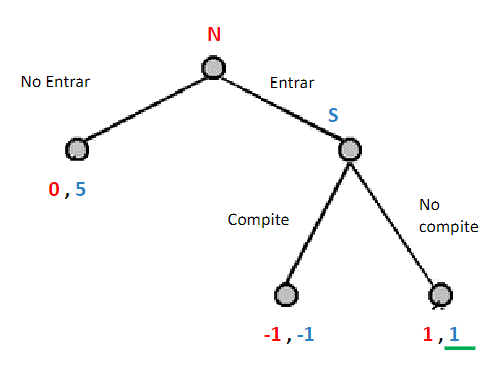
\includegraphics[width=0.5 \linewidth]{figs/secuenciales.png}
                \end{center}
                Notar que las mejores respuestas se pueden identificar mediante la \emph{inducción hacia atrás}. Antes de usarla, debo sabe que la racional secuencial es un hecho: los jugadores son racionales cada vez que les toque jugar.
                
                Comienzo evaluando lo que pasa en los últimos nodos, hasta llegar al nodo inicial.

                Luego de identificar las estrategias óptimas llegamos al ENPS del juego. \\
                \\
                Desafortunadamente para Sony, no hay una forma creíble de comprometerse a competir por precios. Bajar el precio para eliminar al rival del mercado es una estrategia costosa. Por eso el único ENPS de este juego es (E, NC).
            \subsubsection*{Información}
                El \textbf{conjunto de información} indica cuánto saben los jugadores sobre lo que pasó en un juego en un momento dado. Un conjunto de información es unitario cuando contiene a un único nodo de decisión. Teóricamente esto significa que el jugador que debe jugar en ese nodo conoce toda la historia pasada del juego. Cuando todos los conjuntos de información de un juego son unitarios decimos que se trate de un juego de información perfecta (como el problema de la firma entrante). \\
                \\
                Un juego con información perfecta puede ser algo como esto: \\
                \begin{center}
                    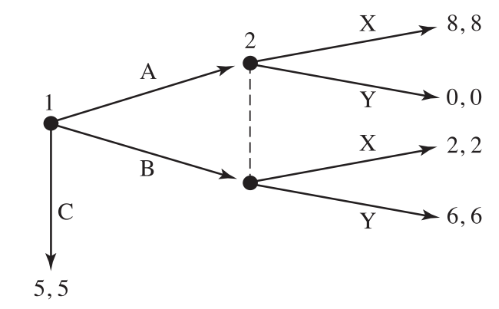
\includegraphics[width=0.5 \linewidth]{figs/informacion.png}
                \end{center}
                Cuando llaman a jugar al jugador 2, este no sabe qué decisión tomó el jugador 1, si A o B. Por eso está con lineas punteadas. \\
                El jugador 1 y el jugador 2 tienen un único conjunto de información. El conjunto de información del jugador 1 es unitario y el conjunto de información del jugador 2 tiene dos nodos de decisión.

                Las acciones para el jugador 2 (X, Y) son las mismas en los dos nodos porque ya no puede diferenciarlos.
            \subsubsection*{Subjuego}
                Un \textbf{Subjuego} es un subconjunto de una forma extensiva que cumple con lo siguiente:
                \begin{itemize}
                    \item Comienza en un conjunto de información unitario.
                    \item Contiene a todos sus nodos sucesores.
                    \item No contiene conjuntos de información imperfecta.
                \end{itemize}
                Un perfil de estrategias (una para cada jugador) conforma un \textbf{equilibrio de Nash perfecto en subjuegos} si me lleva a un equilibrio de Nash en cada subjuego. Cada jugador debe elegir su acción óptima en cada escenario que podría enfrentar, ya que sea que espero que ese escenario ocurra o no.

                Esto me permitirá encontrar Equilibrios de Nash en juegos secuenciales con información perfecta e imperfecta.

                Para encontrar los ENPS hay que hacer la inducción para atrás. \\
                \\
                Presento un caso en el que tenemos tres subjuegos dentro de un único juego. \\
                En el juego \textbf{pasar el sombrero} juegan dos jugadores:
                \begin{itemize}
                    \item Estrategias del jugador 1: poner \$0, \$1 o \$3 en un sombrero. Si el jugador 1 elige \$0, el juego se termina con pagos iguales a cero para ambos jugadores.
                    \item De lo contrario, el sombrero se pasa al jugador 2. Las estrategias del jugador 2 son: “Match” (es decir, agregar la misma cantidad de dinero en el sombrero) o “Take” (tomar el dinero en efectivo).
                    \item Cuando el jugador 2 elige “Take”, se queda con el dinero del J1.
                    \item Cuando el jugador 2 elige “Match” se producen los siguientes pagos netos:
                    \subitem \$1: El J1 recibe pagos netos de \$1, mientras que el J2 recibe pagos netos de \$1,5.
                    \subitem \$3: El J1 recibe pagos netos de \$3, mientras que el J2 recibe pagos netos de \$2.
                \end{itemize}
        \subsection*{Clase VIII: Juegos Secuenciales/Dinámicos (Parte 2)}
            \subsubsection*{Negociación}
                Presento el \textbf{juego del ultimátum con estrategias continuas}.
                \begin{itemize}
                    \item Juegan dos jugadores, J1 y J2.
                    \item Se le entrega la plata a uno de los dos jugadores.
                    \item El jugador que recibe la plata $x$ debe decidir cuánto darle al otro jugador.
                    \item El otro jugador decide si aceptar o no la plata.
                    \item Si acepta la oferta, el J1 recibe $1-x$ mientras que el J2 recibe $x$.
                    \item Si rechaza la oferta, ninguno de los dos se queda con la plata.
                \end{itemize}
                \begin{center}
                    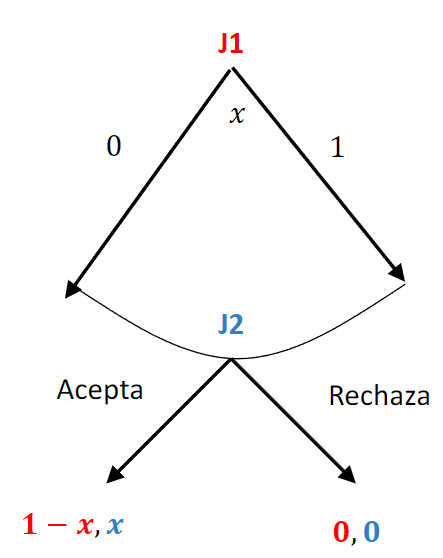
\includegraphics[width=0.3 \linewidth]{figs/ultimatum.png}
                \end{center}
                \begin{enumerate}
                    \item Debo comprender los subjuegos del ejercicio.
                    \subitem La estrategia del J2 une cada posible estrategia $x$ del J1 al conjunto (Aceptar/Rechazar).
                    \subitem J2 tiene un número infinito de conjuntos de información, cada uno para cada una de las ofertas factibles del J1.
                    \subitem La estrategia del J2 tiene que asignar una acción Aceptar/Rechazar a cada una de las infinitas posibles estrategias de J1.
                    \item Resolver por inducción hacia atrás, comenzando por el J2 que debe comparar sus pagos entre aceptar y rechazar en función de $x$.
                    \subitem Tenemos que la estrategia del J2 es:
                    \[
                        E_{2}(x) =
                        \begin{cases} 
                            \text{Aceptar} & \text{si } x \geq 0 \\ 
                            \text{Rechazar} & \text{si } x < 0
                        \end{cases}
                    \]
                    \subitem Sabiendo eso, el J1 ofrecerá $x = 0$, por lo cual el equilibrio perfecto en subjuegos es \((\text{J1:} x = 0; \text{J2: "Aceptar si } x \geq 0 \text{"})\)
                \end{enumerate}
        \subsection*{Clase IX: Juegos Secuenciales/Dinámicos (Parte 3)}
            \textit{La verdad, no sé qué más escribir de esta diapositiva que no haya hecho antes.}
    \section*{\underline{Módulo 4: Juegos Repetidos}}
        \subsection*{Clase X: Juegos Repetidos Finitos}
            \subsubsection*{Aclaraciones}
                En general, las relaciones entre los jugadores duran más que un juego. \\
                Como existe el futuro, nos importa la reputación, los incentivos y los castigos.

                Las relaciones de trabajo duran varios años, las relaciones entre los países surgen de varias instancias de negociación y los competidores en la industria se encuentran muchas veces en el mercado. \\
                Los agentes toman decisiones condicionados por el pasado. Las decisiones futuras estarán influenciadas por lo que va a pasar hoy.
            \subsubsection*{Juegos Repetidos}
                Presento el juego de \textbf{Sticks and Carrots}. \\
                La promesa de recompensas futuras (zanahorias) y la amenaza de castigos futuros (palos) puede proporcionar incentivos a comportarme de forma cooperativa hoy.
                \begin{table}[H]
                    \centering
                        \begin{tabular}{|c|c|c|}
                                & C     & D     \\
                            C   & 5, 5  & 0, \ulcolor[blue]{6}  \\
                            D   & \ulcolor[Red]{6}, 0  & \ulcolor[Red]{1}, \ulcolor[blue]{1}  \\
                        \end{tabular}
                    \caption{Juego de Sticks and Carrots}
                \end{table}
                Este juego se repite dos veces, y es simultáneo en cada período. Cada acción tomada en cada período es independiente. \\
                Los jugadores quieren maximizar los pagos totales en los dos períodos. \\
                Los pagos a futuro no se descuentan ($\delta = 1$). \\
                \\
                El incentivo a cooperar se relaciona con la posibilidad de aumentar mis pagos en el futuro. En la última etapa del juego (t = 1) no hay etapas futuras a tener en cuenta, por lo tanto, espero que en t=1 se juegue (D, D) independientemente de lo que pasó en t=0. \emph{Esto sólo pasa si el juego de tipo Dilema del Prisionero se repite un número finito de veces.} \\
                Resuelvo la etapa cero (t = 0) por inducción hacia atrás, sumando 1 al pago de cada uno de los jugadores sobre el juego inicial.
                \begin{table}[H]
                    \centering
                        \begin{tabular}{|c|c|c|}
                                & C     & D     \\
                            C   & 6, 6  & 1, \ulcolor[blue]{7}  \\
                            D   & \ulcolor[Red]{7}, 1  & \ulcolor[Red]{2}, \ulcolor[blue]{2}  \\
                        \end{tabular}
                    \caption{Juego de Sticks and Carrots modificado}
                \end{table}
                La respuesta sigue siendo la misma. En el último período, $n$, independientemente de lo jugado en las rondas anteriores, existe un único EN para los subjuegos resultantes donde cada jugador juega D. \\
                Las acciones en el anteúltimo período ($n-1$) no tienen ningún efecto en lo que se jugará en el último período. Si vamos para atrás una y otra vez hasta el período inicial, t = 0, nos vamos a enterar que se va a jugar D en cada período.
            \subsubsection*{Cooperación}
                En cada etapa del juego se usa una matriz distinta.
                \begin{table}[H]
                    \centering
                        \begin{tabular}{|c|c|c|}
                                & C     & D     \\
                            C   & 5, 5  & 0, 6  \\
                            D   & 6, 0  & 1, 1  \\
                        \end{tabular}
                    Etapa 1: Dilema del Prisionero
                        \begin{tabular}{|c|c|c|}
                                & S     & R     \\
                            S   & 4, 4  & 0, 2  \\
                            R   & 2, 0  & 2, 2  \\
                        \end{tabular}
                    Etapa 2: Caza del Ciervo                
                \end{table}
                Si propusiera la siguente estrategia: “Juega a Cooperar (C) en la Etapa 1. Si tu compañero también eligió Cooperar (C), juegue Ciervo (S: Stag) en la Etapa 2. Si tu compañero no eligió cooperar (D), juegue Conejo (R: Rabbit) en la segunda etapa”. \\
                ¿Es sostenible esta estrategia?
                \begin{table}[H]
                    \centering
                        \begin{tabular}{|c|c|c|}
                                & C         & D         \\
                            C   & 5+4, 5+4  & 0+2, 6+2  \\
                            D   & 6+2, 0+2  & 1+2, 1+2  \\
                        \end{tabular}
                        \\
                        \begin{tabular}{|c|c|c|}
                                & C     & D     \\
                            C   & 9, 9  & 2, 8  \\
                            D   & 8, 2  & 3, 3  \\
                        \end{tabular}             
                \end{table}
                Los pagos de cooperar son: 5+4 = 9, y los pagos de desviarse son: 6+2 = 8. \\
                \\
                Se puede alcanzar la cooperación en la primera etapa porque uno de los EN es (CS, CS). Para alcanzarlo, la decisión del juego en el futuro debe ser variable (sujeta a lo que sucedió en el pasado).

                Si no hay cooperación, se alcanza igual un EN = (DR, DR). Aún así, la estrategia cooperativa primero (C, C) puede requerir jugar un EN “malo” en la segunda etapa, como lo es (R, R)
        \subsubsection*{Juegos Repetidos Infinitos}
            En un juego finito, en la última etapa siempre se juega un EN. Si no hay (o no sé si hay) una etapa final pasa algo distinto. \\
            \\
            Sabemos que ganar \$1 hoy no es lo mismo que ganar \$1 mañana. El costo de oportunidad hace que un peso invertido hoy me genera $1+r$ mañana por la tasa de retorno.

            Los pagos de los distintos períodos se tienen que expresar en \emph{valor presente} para tomar la decisión correcta. \\ 
            El \textbf{factor de descuento} se define como: \(\delta = \frac{1}{1+r}\). Se sabe que \(0 < \delta < 1\). 

            El $\delta$ será más alto cuanto menor sea la impaciencia, es decir, cuanto más importe el futuro. Al ser más impaciente, le voy a dar una valuación más baja a mis pagos en los períodos futuros. \\
            \\
            En un juego repetido de manera infinita, no se puede sumar de manera infinita los pagos. Acá, \emph{los jugadores deciden en función del valor presente} de los pagos.

            Para el factor de descuento $\delta$ y el vector de pagos \(\pi = (\pi_{0}, \cdots, \pi_{t}, \cdots)\) el valor presente de una secuencia de pagos es:
            \[VP(\pi, \delta) = \pi_{0} + \delta \pi_{1} + \cdots + \delta^{t}\pi_{t} + \cdots\]
            En los juegos infinitos no podemos usar la inducción hacia atrás. \\
            \\
            Si tengo un juego del Dilema del Prisionero repetido infinitamente:
            \begin{table}[H]
                \centering
                    \begin{tabular}{|c|c|c|}
                          & C    & D    \\
                        C & 5, 5 & 0, 6 \\
                        D & 6, 0 & 1, 1 \\
                    \end{tabular}            
            \end{table}
        \subsubsection*{Estrategia Grim-Trigger (Castigo Eterno)}
            Si uso esta estrategia, se comienza jugando C en t = 0. \\
            Se sigue jugando C siempre y cuando los dos hayan jugado C en el período anterior. \\
            Si algún jugador no jugó C en el período anterior, es decir, se desvía, entonces los jugadores jugarán D para siempre. \\
            \begin{center}
                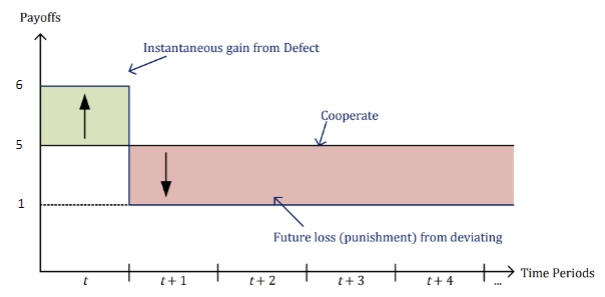
\includegraphics[width=0.75 \linewidth]{figs/grim-trigger.png}
            \end{center}
        \subsubsection*{Estrategia Trigger (Castigo Eterno)}
            ¿Me conviene cooperar si el otro jugador también juega la estrategia trigger? Esto se responderá de forma afirmativa si el pago por cooperar es mayor al pago del desvío. \\
            \\
            Si coopero, obtengo \$5 porque \[5 + \delta 5 + \delta^{2}5 + \cdots = \frac{5}{1-\delta}\]
            Si hay desvío, obtengo \$6 una sola vez, pero luego consigo \$1 siempre porque \[6 + \delta 1 + \delta^{2}1 + \cdots = 6 + 1\frac{\delta}{1-\delta}\]
            Por lo tanto, me convendrá cooperar si: \[\frac{5}{1-\delta} \geq 6 + 1\frac{\delta}{1-\delta}\] \[\therefore \delta \geq \frac{1}{5}\]
            Si adopto la estrategia Trigger, si los dos jugadores son suficientemente pacientes, es decir, \(\delta \geq \frac{1}{5}\), podrán alcanzar el óptimo (5, 5), en vez de llegar al resultado del Dilema del Prisionero del juego de un período. \\
            \\
            Si son suficientemente pacientes los jugadores, ese no es el único equilibrio que se puede alcanzar. Si los jugadores juegan (D, D) en todos los períodos de tiempo también se puede considerar un resultado de equilibrio para todos los valores de $\delta$.
        \subsubsection*{Estrategia Forgiving Trigger (Castigo Temporario)}
            Se comienza jugando C en t = 0. \\
            Se seguirá jugando C, siempre y cuendo los dos jugadores hayan jugado C en el período anterior. \\
            Si algún jugador no jugó C en el período anterior, los dos jugadores jugarán D por una cantidad $k$ de veces. \\
            En el período $k+1$ volverán a cooperar. \\
            \\
            Si el castigo en el juego se da por dos períodos, es decir, $k = 2$, ¿se podrá alcanzar la cooperación si $\delta = \frac{1}{5}$?¿y con $\delta = \frac{3}{5}$?
            \begin{table}[H]
                \centering
                    \begin{tabular}{|c|c|c|}
                          & C    & D    \\
                        C & 5, 5 & 0, 6 \\
                        D & 6, 0 & 1, 1 \\
                    \end{tabular}            
            \end{table}
            Ahora soy el jugador 1. Sé que cooperamos en t = 0. ¿Me convendrá seguir cooperando? \\
            \\
            Si coopero, obtengo \$5 siempre porque \(5 + \delta 5 + \delta^{2}5 + \cdots\) \\
            Si hay desvío, obtengo \$6 una sola vez, pero luego consigo \$1 por dos períodos y vuelvo a conseguir \$5 siempre porque \(6 + \delta 1 + \delta^{2}1 + \delta^{3}5 + \delta^{4}5 + \cdots\) \\
            \\
            Me conviene cooperar si:
            \[5+ \delta 5 + \delta^{2}5 \geq 6 + \delta 1 + \delta^{2}1\]
            \[-1 + 4 \delta + 4 \delta^{2} \geq 0\]
            Si \(\delta = \frac{1}{5} = 0,2\), reemplazo:
            \[-1+4\frac{1}{5}+4(\frac{1}{5})^{2} \geq 0\]
            \[-1+0,2+0,16 \geq| 0\]
            \[-0,04 \geq 0 \implies \text{No se cumple la desigualdad}\]
            Si \(\delta = \frac{3}{5} = 0,6\), reemplazo:
            \[-1+4\frac{3}{5}+4(\frac{3}{5})^{2} \geq 0\]
            \[-1+2,5+1,44 \geq 0\]
            \[2,84 \geq 0 \implies \text{Se cumple la igualdad}\]
            Cuando $k = 2$, un nivel de impaciencia de $\delta = \frac{1}{5}$ no alcanza para sostener el acuerdo. Para que el acuerdo con dos períodos de castigo sea sostenible necesitamos que los jugadores sean más pacientes. Con $k = 2$ necesitamos aproximadamente una tasa de impaciencia de al menos $\delta = 0,21$.

            La posibilidad de conseguir un acuerdo depende de la tasa de impaciencia $\delta$ y de la dureza del castigo $k$.
\end{document}